\begingroup
%\dominitoc
%\faketableofcontents

\let\clearpage\relax

\chapter{Markov Decision Process}
\label{ch:mdp}

%\minitoc

In this chapter, we define the notion of Markov decision process (MDP), a generic model to solve Markovian bandit problem that we will describe in Chapter~\ref{ch:mb}.
MDP is also used to mathematically describe the environment in the Reinforcement Learning (RL) framework.
An MDP models a discrete-time decision problem where the decision maker executes available ``action'' over time steps and receives an immediate incentive known as ``reward'' for each time step.
In such a problem, the decision maker seeks to maximize the expected cumulative rewards by identifying a sequence of actions that produce such an effect.

%The reader who is familiar with MDP can go directly to Section~\ref{ch:mdp:sec:bell} which is a pillar of our contribution in Chapter~\ref{ch:index_computation}.
In Section~\ref{ch:mdp:sec:defn}, we lay out the notation of MDP's parameters and the dynamic of the decision process.
Then, in Section~\ref{ch:mdp:sec:finite}, we briefly present the finite-horizon setting.
Similarly, we present the classical settings for the infinite horizon in Sections~\ref{ch:mdp:sec:discounted} and \ref{ch:mdp:sec:gain}.
%Finally, we introduce a new notion of optimality for infinite horizon setting in Section~\ref{ch:mdp:sec:bell}.


\section{Definitions and notations}
\label{ch:mdp:sec:defn}

In this section, we give the \emph{formalism} of Markov decision process. % and present several notations of \emph{optimality}.
%We also lay out existing results (see \cite{puterman2014markov}) that are pillar of our contribution.
We essentially follow the notations of \cite{puterman2014markov}.

\subsection{State, action, reward, and state transition}

A Markov decision process $M$ is defined as a $4$-tuple $M:=\langle\gS, \gA, r, p\rangle$.
$\gS$ and $\gA:=\cup_{s\in\gS}\gA_s$ denote the \emph{state} and \emph{action} space of the MDP.
When the MDP is in state $s\in\gS$, the decision maker can execute one of the available actions in $\gA_s$.
As a result of executing action $a\in\gA_s$ in state $s$, the MDP incurs a random \emph{reward} with the \emph{expected value} $r(s,a)$ and then transitions to a new state $s'\in\gS$ with probability $p(s'\mid s, a)\in[0,1]$, where $\sum_{s'\in\gS}p(s'\mid s,a)=1$.
The name \emph{Markov} comes from the fact that the random reward and the next state depend only on state $s$ and action $a$ and are independent of anything else.
This thesis considers the MDPs with \emph{finite} state and action spaces, $\abs{\gS}=:S\in\sN$, and $\abs{\gA}=:A\in\sN$.

%\begin{figure}[ht]
%    \centering
%    \begin{tikzpicture}[on grid, state/.style={circle,draw}, >= stealth', auto, prob/.style = {inner sep=1pt,font=\scriptsize}]
%        \node[state,color=blue]  (A) {$s_1$};
%        \node[state,color=blue]  (B) [left =3cm of A]   {$s_0$};
%        \path[->]
%            (A) edge[loop above, color=black] node{$a_1$} (A)
%            (A) edge[loop right, color=red, dashed] node{$a_0$} (A)
%            (B) edge[bend left, color=black] node{$a_1$} (A)
%            (B) edge[bend right, color=red, dashed] node[below]{$a_0$} (A);
%    \end{tikzpicture}
%    \caption{Graphical representation of an MDP with $2$ states ($s_0$ and $s_1$) and 2 actions per state (black arrow and red dashed arrow). We have $p(s_0\mid s_0,a_0)=0, p(s_1\mid s_0,a_0)=1$ and so on.}
%    \label{fig:MDP_example}
%\end{figure}

\subsection{Sequential decision problem and policy}

In this thesis, the decision maker executes actions at \emph{discrete} time steps.
We denote a decision time by $t\in\N^+$ where $\N^+:=\N\setminus\{0\}$ is the set of positive natural numbers.
At time step $t\ge1$, the MDP is in state $s_t$, and the decision maker executes an action $a_t$.
The MDP incurs a (random) reward denoted by $r_t$ and transitions to the next state denoted by $s_{t+1}$.
This mechanism is repeated, and one obtains a sequence of the form $\{s_1,a_1,r_1,s_2,\dots,s_t,a_t,r_t,s_{t+1},\dots\}$ that is called \emph{history} (also known as a ``trajectory'').
%We denote the observations up to time $t\ge1$ by
%\begin{align*}
%    O_t:=\{s_1,a_1,r_1,s_2,\dots,s_{t-1},a_{t-1},r_{t-1},s_t\}
%\end{align*}
%with a convention that $O_1:=\{s_1\}$.
%A \emph{deterministic decision rule} $d$ is a function that maps the observations up to time $t$ to available actions at decision time $t$ with certainty, $d(O_t)\in\gA$.
%The decision rules that depend on previous observations $\gO_t$ only through the current state $s_t$ of the MDP are called \emph{Markovian} decision rule, $d:\gS\mapsto\gA$.

%In this thesis, we restrict our attention to \emph{deterministic Markovian decision rule} and a policy $\pi:=\{d_1,d_2,\dots\}$ is a sequence of deterministic Markovian decision rules for each time step such that at time $t\ge1$, the decision maker follows policy $\pi$ by executing the action $d_t(s_t)\in\gA$. 
A \emph{deterministic decision rule} $\pi$ is a mapping function from state space $\gS$ to action space $\gA$ where for each $s\in\gS$, $\pi(s)\in\gA_s$.
A \emph{policy} is a sequence of deterministic decision rules $\{\pi_1,\pi_2,\dots\}$ such that at time step $t\ge1$, the decision maker follows the policy by executing the action $\pi_t(s_t)\in\gA$.
With a slight abuse of notation, we also denote a policy by $\pi=\{\pi_1,\pi_2,\dots\}$.
We denote the set of all policies by $\Pi$.
%A \emph{stationary} policy is a sequence of decision rules $\{d_t\}_{t\ge1}$ where $d_t=d$ for all $t\ge1$ and $d:\gS\mapsto\gA$ is a mapping function from state space to action space.
We say that a policy is \emph{stationary} when the decision rules are invariant over time step, $\pi_t=\pi$ for all $t\ge1$ and $\pi:\gS\mapsto\gA$.
%By abuse of notation, we will write $d$ and $\pi$ \emph{interchangeably} in the rest of the thesis when policy $\pi=\{d, d,...\}$ is stationary.

The state of the MDP at time step $1$ is called the \emph{initial state} and is generally drawn from a probability distribution $\rho$ such that $\sum_{s\in\gS}\rho(s)=1$.
Given the initial state $s_1$, a policy $\pi\in\Pi$ incurs a sequence $\{s_1,a_1,r_1,\dots,s_t,a_t,r_t,\dots\}$ which is a \emph{stochastic process} with a well-defined probability distribution \cite[Section~2.1.6]{puterman2014markov}.
We will denote by $\sP^\pi(\cdot\mid s_1)$ the \emph{probability measure} associated with this stochastic process and denote by $\mathbb{E}^\pi[\cdot \mid s_1]$ the corresponding \emph{expectation}.

In the following sections, we specify the objective function of the decision problem.

\section{Finite horizon problem}
\label{ch:mdp:sec:finite}

In the finite-horizon setting, the decision maker can collect rewards from an MDP $M$ over a \emph{fixed} number of time steps $H\in\N^+$ called the \emph{horizon}.
We call the expected cumulative reward when following a policy $\pi$ as the \emph{value function}.
That is, the value of state $s$ when starting at time step $1\le h\le H$ and following policy $\pi$ is given by $w_{h:H}^\pi(s){:=}\E^\pi\Bigl[\sum_{t=h}^H r_t\mid s_h{=}s\Bigr]$.
Formally, the decision maker wants to find a policy that satisfies
\begin{equation}
    \label{eq:finite_obj}
    \sup_{\pi\in\Pi}\sum_{s\in\gS}\rho(s)w_{1:H}^\pi(s).
\end{equation}
%From \cite[Chapter~4]{puterman2014markov}, there always exists a sequence of \emph{optimal} policies $\{\pi_1^*,\pi_2^*,\dots,\pi^*_H\}$ that maximizes \Eqref{eq:finite_obj} for any $\rho$ and such that for all $1\le t\le H$, $d_t^*$ is a deterministic Markovian decision rule and independent of the initial state distribution.
From \cite[Chapter~4]{puterman2014markov}, there always exists an \emph{optimal} policy $\pi^*=\{\pi_1^*,\pi_2^*,\dots,\pi^*_H\}$ that maximizes \Eqref{eq:finite_obj} for any $\rho$ and such that for all $1\le h\le H$, $\pi_h^*:\gS\mapsto\gA$ is a deterministic decision rule and independent of the initial state distribution.
For each state $s$, we denote the \emph{optimal} expected cumulative reward from $s$ over time steps $h$ to $H$ by $w_{h:H}^{*}(s){:=}\max_{\pi\in\Pi}w_{h:H}^\pi(s)$.
The maximum value of \Eqref{eq:finite_obj} is given by $\sum_{s\in\gS}\rho(s)w_{1:H}^*(s)$.

From \cite[Chapter~4]{puterman2014markov}, the Bellman \emph{optimality} equations in this setting are written: for $1\le h\le H-1$ and $s\in\gS$,
\begin{equation}
    \label{eq:finite_be_opt}
    w_{h:H}^{*}(s) = \max_{a\in\gA_s}\Big(r(s,a)+\sum_{s'\in\gS}p(s'\mid s,a)w_{h+1:H}^{*}(s')\Big)
\end{equation}
and $w_{H:H}^{*}(s) =\max_{a\in\gA_s}r(s,a)$.
%For a given policy $\pi=\{d_1,\dots,d_H\}$, for each state $s$, we define the expected cumulative reward from $s$ over time steps $h$ to $H$ when following policy $\pi$ by $W_{M,h:H}^\pi(s){:=}\E^\pi\left[\sum_{t=h}^H r_t\mid s_h{=}s\right]$.
%The Bellman \emph{optimality} equations in this setting are written: for $1\le h\le H-1$,
%\begin{equation}
%    \label{eq:finite_be_opt}
%    W_{M,h:H}^{\pi^*}(s) = \max_{a\in\gA_s}\p{r(s,a)+\sum_{s'\in\gS}p(s'\mid s,a)W_{M,h+1:H}^{\pi^*}(s')}
%\end{equation}
%and $W_{M,H:H}^{\pi^*}(s) =\max_{a\in\gA_s}r(s,a)$.
%The function $W_{1:H}$ is the expected cumulative reward from time step $1$ to $H$.
%Suppose that at time step $1\le h\le H$, a policy $\pi$ executes action $a=d_h(s)$ in state $s$ where $a\in\gA_s$.
%Then, the Bellman \emph{evaluation} equation in this setting is
%\begin{equation}
%    \label{eq:finite_be_eval}
%    W_{M,h}^{\pi}(s) = r(s,a)+\sum_{s'\in\gS}p(s'\mid s,a)W_{M,h+1}^{\pi}(s')
%\end{equation}
%with a convention that $W_{H+1}=0$.
So an optimal policy $\pi^*$ can be constructed using backward induction on \Eqref{eq:finite_be_opt}: for each state $s$
\begin{itemize}
    \item $\pi^*_H(s)=\argmax_{a\in\gA_s}r(s,a)$;
    \item for $h$ from $H-1$ to $1$, $\pi^*_h(s)=\argmax_{a\in\gA_s}\Big(r(s,a)+\sum_{s'\in\gS}p(s'\mid s,a)w_{h+1:H}^{*}(s')\Big)$
\end{itemize}
where the ties are broken arbitrarily.
%\begin{algorithm}[ht]
%    \DontPrintSemicolon
%    \SetKwInOut{Input}{Input}\SetKwInOut{Output}{Output}
%    \Input{a MDP $M=\langle\gS,\gA,r,p\rangle$ and horizon $H$}
%    \Init{}{Set $u_{H+1}(s)=0$ for all $s\in\gS$}
%    \BlankLine
%    \For{$h=H$ to $1$}{
%        Set $d_h^*(s) := \displaystyle\argmax_{a\in\gA_s}\Big(r(s,a)+\sum_{s'\in\gS}p(s'\mid s,a)u_{h+1}(s')\Big)$ \tcp{ties are broken arbitrarily} \;
%        Set $u_{h}(s) = \displaystyle r\big(s, d_h^*(s)\big) +\sum_{s'\in\gS}p\big(s' \mid s, d_h^*(s)\big)u_{h+1}(s). \label{eq:finite_be_eval2}$
%    }
%    \Return $\pi^*=\{d_1^*,\dots,d_H^*\}$ and $\vu_1$
%    \caption{Backward Induction}
%    \label{algo:backward}
%\end{algorithm}
%By \cite[Theorem~4.5.1]{puterman2014markov}, Algorithm~\ref{algo:backward} computes an optimal policy and the maximum value of \Eqref{eq:finite_obj} is given by $\sum_{s\in\gS}\rho(s)u_{1}(s)$ where $\vu_1$ is the second output of the algorithm.
%Note that the last part of Equations~\eqref{eq:finite_be_eval1} and \eqref{eq:finite_be_eval2} are known as Bellman \emph{evaluation} equations.

%The backward induction has $\landauO(H\abs{\gS}^2\abs{\gA})$ computational complexity because for each time step, state, and action, the inner product between $p$ and $\vu$ costs $\abs{\gS}$ multiplications at worst.

%\KK{Add Bellman evaluation equations}

Finally, from \cite[Chapter~4]{puterman2014markov} the value function also satisfies the Bellman \emph{evaluation} equations: given a policy $\pi$, for $1\le h\le H$ and $s\in\gS$,
\begin{equation}
    \label{eq:finite_be_eval}
    w_{h:H}^\pi(s) = \displaystyle r\Big(s, \pi_h(s)\Big) +\sum_{s'\in\gS}p\Bigl(s' \mid s, \pi_h(s)\Bigr)w_{h+1:H}^\pi(s')
\end{equation}
with $w_{H+1:H}^\pi(s)=0$.
%\section{Infinite horizon problems}
%
%Similar the previous section, we describe two settings for infinite horizon and provide detail about the optimality criteria in this section.

\section{Infinite horizon discounted problem}
\label{ch:mdp:sec:discounted}

In some problems, the decision maker can collect rewards over an infinite number of time steps, and the immediate reward incurred by the MDP is more critical than those rewards in the future time steps.
To capture this aspect, one can introduce a discount factor denoted by $\gamma$ where $\gamma\in[0,1)$.
If $\gamma=0$, the decision maker is solely interested in the immediate reward from the current state of the MDP.
The value of state $s$ when following a policy $\pi$ is defined by $v^\pi_{\gamma}(s):=\E^\pi\Bigl[\sum_{t=1}^{+\infty} \gamma^{t-1}r_t \mid s_1=s\Bigr]$.
It captures the cumulative discounted reward one would expect when starting from state $s$ and following policy $\pi$.
The decision maker wants to find a policy that satisfies
\begin{equation}
    \label{eq:discount_obj}
    \sup_{\pi\in\Pi}\sum_{s\in\gS}\rho(s)v^\pi_{\gamma}(s).
\end{equation}
From \cite[Chapter~6]{puterman2014markov}, there always exists a stationary optimal policy $\pi^*:\gS\mapsto\gA$ that maximizes \Eqref{eq:discount_obj} for any initial distribution $\rho$.
%For a given stationary policy $\pi:\gS\mapsto\gA$, the expectation in \Eqref{eq:discount_obj} is known as the \emph{value} of state $s$ under policy $\pi$ and denoted by $v^\pi(s)$.
For any $s$, since $0\le\gamma<1$, $v_\gamma^\pi(s)$ is a geometric series that converges.
So, $v^\pi_\gamma(s)$ exists and is well-defined for any state $s$ and any policy $\pi\in\Pi$.
The value function of policy $\pi$ satisfies the following Bellman evaluation equation: for each $s\in\gS$
\begin{equation}
    \label{eq:discount_be_eval}
    v^\pi_\gamma(s) =r\bigl(s,\pi(s)\bigr) +\gamma\sum_{s'\in\gS}p\bigl(s'\mid s,\pi(s)\bigr)v^\pi_\gamma(s').
\end{equation}
The \emph{optimal} value function is defined by $v^*_\gamma(s):=\max_{\pi\in\Pi}v^\pi_\gamma(s)$ for all $s\in\gS$.
By \cite[Theorem~6.2.5]{puterman2014markov}, the optimal value function $\vv^*_\gamma\in\R^{S}$ is unique: any optimal policies induce the same value function.
Moreover, $\vv^*_\gamma$ satisfies the Bellman optimality equation: for each $s\in\gS$
\begin{equation}
    \label{eq:discount_be_opt}
     v^*_\gamma(s)= \max_{a\in\gA_s}\Big(r(s, a) +\gamma\sum_{s'\in\gS}p(s'\mid s,a)v^*_\gamma(s')\Big).
\end{equation}
So, the maximum value of \Eqref{eq:discount_obj} is given by $\sum_{s\in\gS}\rho(s)v^*_\gamma(s)$.
%It is well-known that an optimal policy can be constructed using iterative algorithms such as Value Iteration given in Algorithm~\ref{algo:discounted_vi}.

It is well-known that an optimal policy can be constructed as the following: for all state $s$, $\pi^*(s)=\argmax_{a\in\gA_s}\Big(r(s, a) +\gamma\sum_{s'\in\gS}p(s'\mid s,a)v^*_\gamma(s')\Big)$, where the ties are broken arbitrarily.
This requires the optimal value function $\vv^*_\gamma$, which is approximated by iterative algorithms such as value iteration:
\begin{itemize}
    \item initialize $v_\gamma^0(s)=0$ for all $s\in\gS$
    \item iterate over $k$: $v^{k+1}_\gamma(s) = \max_{a\in\gA_s}\Big(r(s,a)+\gamma\sum_{s'\in\gS}p(s'\mid s,a)v_{\gamma}^k(s')\Big)$ for all $s\in\gS$, then update $k=k+1$ and repeat until $\norm{\vv^{k+1}_\gamma-\vv^k_\gamma}\le(1-\gamma)\varepsilon/\gamma$
\end{itemize}
where $\norm{\cdot}$ can be the maximum norm or span semi-norm on $\R^{S}$, and $\varepsilon$ is the accuracy of the approximation.
From \cite[Chapter~6]{puterman2014markov}, this iterative schema always converges: $\lim_{k\to\infty}\vv^k_\gamma=\vv^*_\gamma$.
Precisely, this schema stops after a finite number of iterations $K$, where $\norm{\vv^K_\gamma-\vv^*_\gamma}\le \varepsilon$ (see \cite[Theorem~6.3.1]{puterman2014markov}). 
%\begin{algorithm}[ht]
%    \DontPrintSemicolon
%    \SetKwInOut{Input}{Input}\SetKwInOut{Output}{Output}
%    \Input{an MDP $M=\langle\gS,\gA,r,p\rangle$, discount factor $\gamma\in[0,1)$, and accuracy $\varepsilon\in(0,1)$}
%    \Init{}{Set $n=0$ and $v_0(s)=0$ for all $s\in\gS$}
%    \BlankLine
%    Set $v_1(s)=\max_{a\in\gA_s} r(s,a)$ for all $s\in\gS$ \;
%    \While{$\displaystyle\max_{s\in\gS}\big(v_{n+1}(s)-v_n(s)\big) -\min_{s\in\gS}\big(v_{n+1}(s)-v_n(s)\big) \ge \frac{1-\gamma}{\gamma}\varepsilon$}{
%        Set $n=n+1$ \;
%        Set $v_{n+1}(s) = \displaystyle\max_{a\in\gA_s}\Big(r(s,a)+\sum_{s'\in\gS}p(s'\mid s,a)v_{n}(s')\Big)$ for all $s\in\gS$
%    }
%    Set $\pi(s):=\displaystyle\argmax_{a\in\gA_s}\Big(r(s,a)+\sum_{s'\in\gS}p(s'\mid s,a)v_{n+1}(s')\Big)$ for all $s\in\gS$ \tcp{ties are broken arbitrarily}\;
%    \Return $\pi$ and $\vv_{n+1}$
%    \caption{Value Iteration}
%    \label{algo:discounted_vi}
%\end{algorithm}
%
%Similar to backward induction, Algorithm~\ref{algo:discounted_vi} has $\landauO(\abs{\gS}^2\abs{\gA})$ computational complexity where $\landauO(\cdot)$ hides the total number of iterations.

This setting with a discount factor $\gamma$ can be seen as a finite-horizon setting whose horizon is randomly sampled from a \emph{geometric distribution} with parameter $(1-\gamma)$.
Precisely, the decision maker can stop interacting with the MDP with probability $(1-\gamma)$ at each time step.
So, the value of state $s$ under stationary policy $\pi$ is the expected sum of rewards over the random horizon:
\begin{equation}
    \label{eq:discount_finite}
    v^\pi_\gamma(s) :=\E^\pi\left[\sum_{t=1}^{+\infty} \gamma^{t-1}r_t \mid s_1{=}s\right] {=}\ex{\E^\pi\bigg[\sum_{t=1}^H r_t\mid H, s_1{=}s\bigg]} =\ex{W^\pi_{1:H}(s)},
\end{equation}
where the expectation of the fourth term integrates over the randomness of the horizon $H$ whose expected value is $1/(1-\gamma)$.

%\subsection{Average reward model}
\section{Infinite horizon average reward criterion}
\label{ch:mdp:sec:gain}

In some problems, the decision maker is more interested in the long-term average reward per decision time than the expected cumulative discounted reward.
Therefore, we focus on this criterion in this section.

\subsection{Gain and bias}

Formally, the decision maker wants to identify a policy that satisfies
\begin{equation}
    \label{eq:avg_obj}
    \sup_{\pi\in\Pi}\sum_{s\in\gS}\rho(s)\liminf_{T\to+\infty}\frac1T \E^\pi\left[ \sum_{t=1}^{T} r_t \mid s_1=s\right].
\end{equation}
Since the state space is finite, the infimum limit of \Eqref{eq:avg_obj} equals the supremum limit for any stationary policy $\pi$ (see \cite[Chapter~8]{puterman2014markov}).
Hence, the limit of \Eqref{eq:avg_obj} exists and is called the \emph{long-term} average reward or \emph{gain} of state $s$ under policy $\pi$.
Concretely, it is defined by
\begin{equation}
    \label{eq:gain_defn}
    g^\pi(s) := \lim_{T\to+\infty}\frac1T \E^\pi\left[ \sum_{t=1}^{T} r_t \mid s_1=s\right].
\end{equation}
This notion generalizes both the finite horizon and the discounted settings when $H\to+\infty$ or $\gamma\to1$ because it is shown (see \cite[Sections~8.2.1 and 8.2.2]{puterman2014markov}) that 
%\begin{align*}
%    \E^\pi\left[\sum_{t=1}^H r_t\mid s_1{=}s\right] \underset{H\to+\infty}{\sim} Hg^\pi(s) \text{ and }
%    \E^\pi\left[\sum_{t=1}^{+\infty} \gamma^{t-1}r_t \mid s_1{=}s\right] \underset{\gamma\to1}{\sim}
%    g^\pi(s)/(1-\gamma).
%\end{align*}
%\begin{align*}
%    w^\pi_{1:H}(s) \underset{H\to+\infty}{\sim} Hg^\pi(s) \text{ and }
%    v^\pi_\gamma(s) \underset{\gamma\to1}{\sim}
%    g^\pi(s)/(1-\gamma).
%\end{align*}
\begin{equation}
    \label{ch:mdp:eq:equi_gain_value}
    \lim_{H\to+\infty}\frac1H w^\pi_{1:H}(s) =g^\pi(s) \text{ and }
    \lim_{\gamma\to1}(1-\gamma)v^\pi_\gamma(s) =g^\pi(s).
\end{equation}
In consequence, if $\pi$ and $\pi'$ are two stationary policies such that $g^\pi(s)< g^{\pi'}(s)$, then for $H$ big enough and $\gamma$ close enough to $1$, $w_{1:H}^\pi(s)< w_{1:H}^{\pi'}(s)$ and $v^\pi_\gamma(s)< v^{\pi'}_\gamma(s)$.
%$\E^\pi\left[\sum_{t=1}^H r_t\mid s_1{=}s\right]\le \E^{\pi'}\left[\sum_{t=1}^H r_t\mid s_1{=}s\right]$ and $\E^\pi\left[\sum_{t=1}^{+\infty} \gamma^{t-1}r_t \mid s_1{=}s\right]\le \E^{\pi'}\left[\sum_{t=1}^{+\infty} \gamma^{t-1}r_t \mid s_1{=}s\right]$.

The gain of a stationary policy captures the average reward obtained in the \emph{steady regime} (or \emph{asymptotic regime}).
Another quantity associated with a stationary policy $\pi$ is its \emph{bias function}, defined by: for each $s\in\gS$
\begin{equation}
    \label{eq:bias_defn}
    h^\pi(s) :=\Clim_{T\to+\infty} \E^\pi\left[ \sum_{t=1}^{T} r_t -g^\pi(s_t) \mid s_1=s\right].
\end{equation}
The \emph{Cesaro-limit} denoted by $\mathrm{C}$-$\mathrm{lim}$ is used because it is well-defined for any stationary policies, albeit the ``classical'' limit may not exist for a stationary policy that induces a stochastic process governed by a \emph{periodic} Markov chain.
The bias function captures the expected total difference between the reward and the average reward in the steady regime. 
The difference of bias values $h^\pi(s)-h^\pi(s')$ captures the (dis-)advantage of starting at state $s$ rather than $s'$ when following policy $\pi$.
We denote by $sp(\vh^\pi):=\max_{s\in\gS}h^\pi(s) -\min_{s\in\gS}h^\pi(s)$ the range or \emph{span} of the bias function of policy $\pi$.

Any stationary policy $\pi$ induces a Markov reward process (MRP), where the reward function and state transition are encoded by vector $\vr^\pi$ and stochastic matrix $\mP^\pi$ such that for any $s,s'\in\gS$, $r^\pi(s):=r\big(s,\pi(s)\big)$ and $P^\pi(s,s'):=p\big(s'\mid s,\pi(s)\big)$.
%We define the \emph{limiting matrix} $\bar{\mP}^\pi:=\Clim_{t\to+\infty}{(\mP^\pi)^t}$ (\cite[Appendix~A.4]{puterman2014markov}). % which describes the state transition in steady regime under policy $\pi$. That is, $\bar{P}^\pi(s,s')$ is the probability that the MDP transitions from state $s$ to $s'$ in steady regime.
%Since the MDP has finite state space, $\bar{\mP}^\pi$ always exists and well-defined for any stationary policy $\pi$.
%It describes the state transition in steady regime under policy $\pi$. That is, $\bar{P}^\pi(s,s')$ is the probability that the MDP transitions from state $s$ to $s'$ in steady regime.
%So, the gain of policy $\pi$ can be expressed by for any $s\in\gS$, $g^\pi(s)=\sum_{s'\in\gS}\bar{P}^\pi(s,s')r^\pi(s')$.
%In vector notation, $\vg^\pi=\bar{\mP}^\pi\vr^\pi$.
%However, computing $\vg^\pi$ through $\bar{\mP}^\pi$ might be inefficient.
%Instead, the gain and bias can be computed using Bellman evaluation equations given in Proposition~\ref{prop:be_eval}.
The gain and bias can be computed using Bellman evaluation equations given in Proposition~\ref{prop:be_eval}.
\begin{prop}[{\cite[Theorem~8.2.6]{puterman2014markov}}]
    \label{prop:be_eval}
    For any stationary policy $\pi$, the gain $\vg^\pi$ and bias $\vh^\pi$ satisfy the following system of Bellman evaluation equations: for any $s\in\gS$
    \begin{align}
        g(s) -\sum_{s'\in\gS}P^\pi(s,s')g(s') &=0 \label{eq:gain_eval}\\
        g(s) -r^\pi(s) +h(s) -\sum_{s'\in\gS}P^\pi(s,s')h(s') &=0. \label{eq:bias_eval}
    \end{align}
    Moreover, suppose that $\vg$ and $\vh$ satisfy \eqref{eq:gain_eval} and \eqref{eq:bias_eval}. Then, $\vg^\pi=\vg$ and $\vh^\pi=\vh+\vu$ where $u(s)=\sum_{s'\in\gS}P^\pi(s,s')u(s')$ for all $s$.
    %Finally, if $\bar{\mP}^\pi\vh=\vzero$, then $\vh^\pi=\vh$.
\end{prop}
Equations~\eqref{eq:gain_eval} and \eqref{eq:bias_eval} uniquely define $\vg$ and determine $\vh$ up to an element of the null space of $(\mI-\mP^\pi)$ where $\mI$ is the identity matrix of size $S\times S$.
If $\mP^\pi$ is unichain\footnote{we provide more explanation about unichain in \ref{it:unichain} of Definition~\ref{ch:mdp:defn:mdp_class}.}, then we say that policy $\pi$ is unichain, and its gain is state independent: $g^\pi(s)=g^\pi(s')$ for any $s,s'\in\gS$.
So, for any policy $\pi$ that is unichain, we just denote its gain by $g^\pi$.
Moreover, if $\pi$ is unichain, its bias vector $\vh^\pi$ is defined up to a constant vector (see \cite[Chapter 8]{puterman2014markov}).

\subsection{Classification of Markov decision processes}
Since \Eqref{eq:avg_obj} compares policies based on their average reward in the steady regime, we need to take into account the chain structure induced by the policies.
%We assume that the reader is familiar with the notion of \emph{transient} and (positive) \emph{recurrent} states and/or class of a Markov chain (see \cite[Appendix~A]{puterman2014markov} or \cite{levin2017markov} for more detail) and classify the MDPs according to the following definition.
In an MDP with a finite state space, the states are either \emph{transient} or \emph{recurrent}.
A state is \emph{transient} if it is never visited in the steady regime.
For more formal definition, the reader may refer to \cite[Appendix~A]{puterman2014markov} or \cite{levin2017markov}.
We classify the MDPs according to the following definition.
\begin{defn}[Classification of MDPs]
    \label{ch:mdp:defn:mdp_class}
    We say that an MDP is
    \begin{enumerate}[label=(\roman*)]
        \item \textbf{ergodic} if the Markov chain induced by any stationary policy has a single recurrent class that coincides the state space (\ie, all states are visited infinitely often with probability $1$ independently of initial state);
        \item \label{it:unichain} \textbf{unichain} if the Markov chain induced by any stationary policy is \emph{unichain}, \ie, it has a single recurrent class plus a --possibly empty-- set of transient states;
        \item \textbf{multichain} if it is not unichain;
        \item \textbf{communicating} if for every pair of states $(s,s')\in\gS$, there exists a stationary policy under which $s'$ is accessible from $s$ in a finite number of time steps with non-zero probability
        \item \textbf{weakly communicating} if the state space can be partitioned into two subsets $\gS^{\gC}$ and $\gS^{\gT}$ (with $\gS^{\gT}$ possibly empty), such that for every pair of states $(s,s')\in\gS^{\gC}$, there exists a stationary policy under which $s'$ is accessible from $s$ in finite time with non-zero probability, and all states in $\gS^{\gT}$ are transient under all stationary policies.
    \end{enumerate}
\end{defn}
With this definition, ergodic MDPs are special cases of unichain MDPs, and weakly communicating MDPs generalize communicating MDPs. 
Moreover, ergodic MDPs are communicating, and unichain MDPs are weakly communicating.
Figure~\ref{ch:mdp:fig:mdp_class} summarizes this relation.

\begin{figure}[ht]
    \centering
    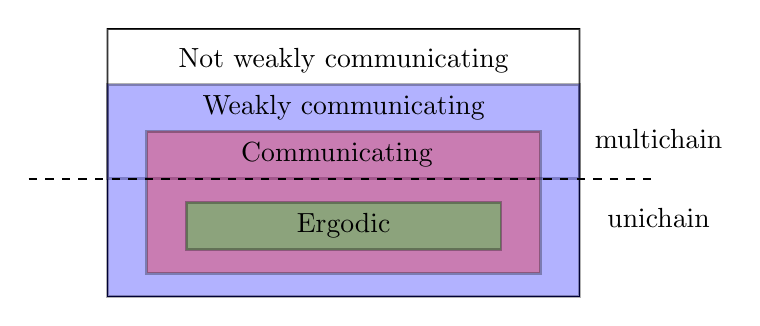
\begin{tikzpicture}
        \draw (0,1) rectangle (6,4.4);
        \node at (7,3) {multichain};
        \node at (7,2) {unichain};
        % \node[text width=2cm, align=center] at (-1.5,0.5) {discounted problems};
        \draw[line width=1pt, fill=white,opacity=0.3] (0,2.5) rectangle (6,4.4);
        \node[text width=5cm, align=center] at (3,4) {Not weakly communicating}; %multichain
        \draw[line width=1pt, fill=blue,opacity=0.3] (0,1) rectangle (6,3.7);
        \node[text width=4cm, align=center] at (3,3.4) {Weakly communicating};
        %\draw[line width=1pt, fill=white,opacity=0.3] (0,1) rectangle (6,2.5);
        %\node{}; %unichain
        \draw[line width=1pt, fill=red, opacity=0.3] (0.5,1.3) rectangle (5.5,3.1);
        \node[text width=2cm, align=center] at (2.7,2.8) {Communicating};
        \draw[line width=1pt, fill=green,opacity=0.3] (1,1.6) rectangle (5,2.2);
        \node[text width=2cm,align=center] at (3,1.9) {Ergodic};
        \draw[line width=0.7pt, dashed] (-1,2.5) -- (7,2.5);%  (-2,1) -- (6.5,1);
    \end{tikzpicture}
    \caption{MDP space: the portion of rectangle below the dashed line represents the set of unichain MDPs, and the portion above the dashed line represents the set of multichain MDPs.
        The blue rectangle is the set of weakly communicating MDPs.
        The red rectangle on top of the blue one is the set of communicating MDPs.
        Finally, the green rectangle on top of the red one is the set of ergodic MDPs.
    }
    \label{ch:mdp:fig:mdp_class}
\end{figure}

Testing if a Markov chain is unichain can be done in $\landauO(S^2)$ using Tarjan's strongly connected component algorithm.
Testing if an MDP is unichain is, however, NP-hard \cite{tsitsiklis2007np}.
%For the pattern of states that are accessible from each other, we can check if a MDP is communicating or weakly communicating in $\landauO(\abs{\gS}^2)$ by leveraging \cite[Proposition~8.3.1]{puterman2014markov}:
%we construct a stochastic matrix $\mP^{\#}$ such that for all $s,s'\in\gS$, $P^{\#}(s,s'):=\displaystyle\frac1{\abs{\gA_s}}\sum_{a\in\gA_s}p(s'\mid s,a)$.
%We check the structure of Markov chain induced by $\mP^{\#}$ using Tarjan's strongly connected component algorithm and draw a conclusion as the following:
%\begin{itemize}
%    \item the MDP is communicating if and only if $\mP^{\#}$ is recurrent;
%    \item the MDP is weakly communicating if and only if $\mP^{\#}$ is unichain. 
%\end{itemize}

\subsection{Gain optimality}
\label{ch:mdp:ssec:gain}

Similarly to the discounted setting, in MDPs with finite state and action spaces, there always exists an optimal stationary policy $\pi^*$ that satisfies \Eqref{eq:avg_obj} for any initial distribution $\rho$ (see \cite[Theorem~9.1.8]{puterman2014markov}).
Such an optimal policy $\pi^*$ induces the \emph{optimal gain} denoted by $\vg^*$, and the value of \Eqref{eq:avg_obj} is given by $\sum_{s\in\gS} \rho(s)g^*(s)$.
From \cite[Chapter~9]{puterman2014markov}, the optimal gain $\vg^*$ satisfies the following system of \emph{modified optimality} equations: for each $s\in\gS$,
\begin{align}
    g(s) &= \max_{a\in\gA_s} \sum_{s'\in\gS}p(s'\mid s,a)g(s') \label{eq:gain_opt} \\
    g(s) +h(s) &= \max_{a\in\gA_s}\Big(r(s,a) +\sum_{s'\in\gS}p(s'\mid s,a)h(s')\Big) \label{eq:bias_opt}.
\end{align}
\cite[Chapter~9]{puterman2014markov} also provides the \emph{optimality} equations for $\vg^*$, but we do not use them in this thesis.
%In this thesis, we only use the modified optimality equations of \cite{puterman2014markov}.
So, we will just call \eqref{eq:gain_opt} and \eqref{eq:bias_opt} the \emph{Bellman optimality} equations.

$\vg^*$ is uniquely defined by \eqref{eq:gain_opt} and \eqref{eq:bias_opt}.
Any policies achieving $\vg^*$ are said to be \emph{gain optimal} (or average reward optimal): for any $\pi\in\Pi$, $g^\pi(s)\le g^*(s)$ for all $s\in\gS$.
By \cite[Theorem~8.3.2]{puterman2014markov}, if an MDP is weakly communicating, then the optimal gain is state independent: $g^*(s)=g^*(s')$ for any $s,s'\in\gS$.
So, in weakly communicating MDPs, we just denote the optimal gain by $g^*$.
Note that the fact that the optimal gain is constant over states does not imply that all gain optimal policies are unichain.
Table~\ref{tab:mdp_vs_gain} describes the gain of stationary policies in different classes of MDPs.
\begin{table}[ht]
    \begin{tabular}{lll}
        \hline
        Model class          & Optimal gain         & Gain of a stationary policy \\ \hline
        Ergodic              & Constant             & Constant                    \\
        Unichain             & Constant             & Constant                    \\
        Communicating        & Constant             & Possibly nonconstant        \\
        Weakly Communicating & Constant             & Possibly nonconstant        \\
        Multichain           & Possibly nonconstant & Possibly nonconstant       \\ \hline
    \end{tabular}
    \caption{\cite[Table~8.3.1]{puterman2014markov}: Relationship between MDP class and gain}
    \label{tab:mdp_vs_gain}
\end{table}
Finally, we denote $\vh^*\in\R^{S}$ the vector that satisfies \eqref{eq:bias_opt} with $\vg^*$.
Equations \eqref{eq:gain_opt} and \eqref{eq:bias_opt} do not uniquely defined $\vh^*$.
The properties of solution space for $\vh^*$ given $\vg^*$ is studied in \cite{schweitzer1978functional}.
%Moreover, we have $\bar{\mP}^\pi\mP^\pi =\mP^\pi\bar{\mP}^\pi =\bar{\mP}^\pi$.
%However, computing $\vg^\pi$ through $\bar{\mP}^\pi$ might be inefficient.

\endgroup
